% TODO:
%
% * email to full collaborator list
% * add any missing CPS coauthors
%
%%%%%%%%%%%%%%%%%%%%%%%%%%%%%%%%%%%%%%%%%%%%%%%%%%%%%%%%%%%%%%%%%%%%%%%%%%%%%%%

\documentclass[12pt,twocolumn,tighten]{aastex62}
\usepackage{amsmath,amstext,amssymb}
\usepackage[T1]{fontenc}
\usepackage{apjfonts}
\usepackage[figure,figure*]{hypcap}
\usepackage{graphics,graphicx}
\usepackage{hyperref}
\usepackage{natbib}

\renewcommand*{\sectionautorefname}{Section} %for \autoref
\renewcommand*{\subsectionautorefname}{Section} %for \autoref

%% Reintroduced the \received and \accepted commands from AASTeX v5.2.
%% Add "Submitted to " argument.
\received{\today}
\revised{---}
\accepted{---}
\submitjournal{AAS journals.}
\shorttitle{WASP-4 is accelerating towards the Earth}

\begin{document}

\defcitealias{bouma_wasp4b_2019}{B19}

% TODO: may want to improve title
\title{WASP-4 is Accelerating Towards the Earth}
% ": A Cautionary Tale in the Search for Tidal Orbital Decay"
% "An Explanation for WASP-4's Decreasing Orbital Period".
% "WASP-4's Decreasing Orbital Period: Solved."

\correspondingauthor{L. G. Bouma}
\email{luke@astro.princeton.edu}

%
% key authors: did Rachel do the Zorro reductions?
%
\author[0000-0002-0514-5538]{L. G. Bouma}
\affiliation{ Department of Astrophysical Sciences, Princeton
University, 4 Ivy Lane, Princeton, NJ 08540, USA}
%
\author[0000-0002-4265-047X]{J. N. Winn}
\affiliation{ Department of Astrophysical Sciences, Princeton
University, 4 Ivy Lane, Princeton, NJ 08540, USA}

%
% contributing authors: alphabetical
%
\author[0000-0002-0531-1073]{H. Isaacson}
\affiliation{Astronomy Department, University of California, Berkeley,
CA 94720, USA}
%
\author[0000-0001-8638-0320]{A. W. Howard}
\affiliation{Cahill Center for Astrophysics, California Institute of
Technology, Pasadena, CA 91125, USA}
%
\author{S. B. Howell}
\affiliation{NASA Ames Research Center, Moffett Field, CA 94035, USA}
%
\author{H. Knutson}
\affiliation{Division of Geological and Planetary Sciences, California
Institute of Technology, Pasadena, CA 91125, USA}
%
%
%\author{R. A. Matson}
% \affiliation{NASA Ames Research Center, Moffett Field, CA 94035, USA}
%

\begin{abstract}
  We recently reported that space and ground-based transit observations
  showed the orbital period of WASP-4b to be decreasing.
  Possible explanations included tidal orbital decay, orbital
  precession, and light-travel time effects.
  In this work we present new observations of the radial velocity of
  WASP-4, acquired with Keck-HIRES.
  The new data show that the system is accelerating towards our line
  of sight, at $\dot{\gamma} = X.XX \pm Y.YY\ {\rm m}\,{\rm
  s}^{-1}\,{\rm yr}^{-1}$.
  This implies a period decrease of X.XX milliseconds per year,
  compared to the observed value of Y.YY.
  Combining the radial velocities with new speckle imaging from
  Gemini-Zorro, we find that the WASP-4 system likely has a
  10-200$\,M_{\rm Jup}$ companion with semi-major axis between 10 and
  100$\,$AU.
  As observing baselines continue to extend, long-term tracking of hot
  Jupiter radial velocities will be necessary to distinguish tidal
  orbital decay from the R{\o}mer delay.
\end{abstract}

\keywords{Exoplanet tides (497), Exoplanet dynamics (490), Radial velocity 
(1332), Transit timing variation method (1710)}

%%%%%%%%%%%%%%%%%%%%%%%%%%%%%%%%%%%%%%%%%%%%%%%%%%%%%%%%%%%%%%%%%%%%%%%%%%%%%%%

\section{Introduction}

Since the first discovery of transiting hot Jupiters, the hunt for
tidal orbital decay has received much attention (CITE LIKE 20 PAPERS).
These efforts are gradually beginning to yield fruit: by combining
transit and occultation timing and radial velocity measurements, CITE
Yee et al{.} have shown that the data for the hot Jupiter WASP-12b are
most compatible with orbital decay.

The present study highlights a point that, while obvious, has perhaps
not yet received due attention.  The point is that the hunt for
orbital decay of hot Jupiters will be crippled without long-term
radial velocity monitoring programs.  The reason is simple: when the
timescale of orbital period change far exceeds the observing baseline,
the first deviation from constant periodicity is always quadratic in
the transit number.

There are ample reasons to expect orbital decay to be common (CITE).
However there are reasons to expect the R{\o}mer delay to perhaps be
even {\it more} common (CITE Knutson 14, Bryan 16).  Both manifest to
first order identically in transit times (up to the sign of the
line-of-sight acceleration) -- as a non-zero period derivative.

Specifically, \citet{knutson_friends_2014} showed that X\% of hot
Jupiters show some form of radial acceleration in radial velocity
time-series with baselines of YY years.  Assuming a separation
distribution of (WHATEVER), this implies that ZZ\% of hot Jupiters
will {\it always} show a changing orbital period, over timescale of
say 10 years.
The abundance of giant planets
exterior to Super-Earth sized systems is also high (CITE Bryan 2019),
but this is not so much of a concern to us, as their planetary masses
and therefore tidal timescales are typically expected to be at least
an order of magnitude shorter than hot Jupiters.

The main focus of this study is the hot Jupiter WASP-4b, which has an
orbital period that from transits appears to be decreasing by about 10
milliseconds per year.  We discovered the timing variations using
data from TESS and a decade of ground-based monitoring
\citep[][hereafter \citetalias{bouma_wasp4b_2019}]{bouma_wasp4b_2019}.

Thereafter, \citet{southworth_transit_2019} reported 22 new transit
times for the system, and confirmed that the updated series of transit
times was consistent with a quadratic ephemeris.  With additional
data, they found a lower best-fit decay rate of $\dot{P} = -XX.X \pm
X.X$ milliseconds per year.

A separate study by \citet{baluev_2019} reported
additional archival transit light curves of WASP-4b, most notably from
the TRAPPIST archive, and a select few other observers.
% \citeauthor{baluev_homogeneously_2019} analyzed their newly obtained
% photometry, along with archival light curves that we omitted from our
% analysis due to systematic uncertainties in the absolute time system.
\citeauthor{baluev_2019} found that when they used all
the available TTV data, the need for a quadratic ephemeris was present
``at the high $\sim 5-7$ sigma level''.  However, they pointed out
that if they used lower-precision subsets of the available timing
data, the necessity for the quadratic term decreased. This is not
particularly surprising.
% \citeauthor{baluev_homogeneously_2019} also pointed out that the
% precise transit times reported by \citet{huitson_gemini_2017} were
% quite important in the time-series.  Overall,
% \citeauthor{baluev_homogeneously_2019} did not find the claim of a
% period decrease convincing.

To determine the origin of the period change, we acquired four
additional radial velocity measurements using Keck-HIRES, extending
the RV baseline from 3 to 9 years.  Previously, the radial velocities
were sparse and showed a weak ($<2\sigma$) linear trend.  Our new
measurements reveal a line of sight acceleration of $\dot{\gamma} =
-XX {\rm m\,s^{-1}\,yr^{-1}}$.  This translates to an expected period
decrease simply from the light travel time effect of ZZ milliseconds
per year --- about commensurate with what is observed.

% FIXME: figure out correct sections
\S~\ref{sec:observations} presents the new observations...
\S~\ref{sec:analysis} describes our analysis...
\S~\ref{sec:discussion} discusses...
\S~\ref{sec:conclusions} gives conclusions...

\section{Observations}
\label{sec:observations}

\subsection{Transits}

{\bf Table~N} lists the transit times we used in our analysis.  We
include data from the peer-reviewed literature for which (a) the
analysis was based on observations of a single transit, (b) the
midpoint was fitted as a free parameter, and (c) the time system
specified both the absolute reference (TDB or UTC) and also whether
any barycentric or heliocentric corrections had been performed.

The majority of times are identical to those we collected in
\citetalias{bouma_wasp4b_2019}.  Twenty-two new times reported by
\citet{southworth_transit_2019} are included.  These transits were
observed from the 3.58m NTT and Danish 1.54m telescopes at La Silla,
and the SAAO 1.0m telescope.

% FIXME : verify with Michael Gillon and Phil Evans that this is true.
A number of additional times were also recently reported by
\citet{baluev_2019}, based on a homogeneous analysis of archival
ground-based observations.  We included their ``high quality'' transit
times with provenance from the TRAPPIST and El Sauce telescopes, for
which we verified with the original observers that appropriate
time-system corrections had been performed (M.~Gillon, P.~Evans,
priv{.} comm{.}).

The four available occultation data points tabulated by
\citetalias{bouma_wasp4b_2019} are sparse and have neglegible
statistical value due to their large uncertainties, and we forgo
their use in this analysis.  

\subsection{Radial velocities}

% TODO: Details of reduction from Howard or Knutson
After identifying the period decrease in
\citetalias{bouma_wasp4b_2019}, we acquired four additional radial
velocity measurements with the Keck High Resolution Echelle
Spectrometer (HIRES, \citealt{vogt_hires_1994}).  Our observations
were acquired under the purview of the California Planet Survey
\citep{howard_cps_2010}.  The spectra were reduced using {\bf software
X}.  Previously, the HIRES data-points spanned 2010 to 2013
\citep{knutson_friends_2014}.  Our new measurements triple the HIRES
observing baseline to nine years.

%FIXME: I should ask Didier if he has any new CORALIE observations...
The complete set of radial velocity observations is given in {\bf
Table~M}.  Along with the 2010-2019 HIRES observations, there are also
earlier measurements from CORALIE and HARPS.  Following
\citetalias{bouma_wasp4b_2019}, we included the CORALIE measurements
from \citet{wilson_wasp-4b_2008} and \citet{triaud_spin-orbit_2010},
using the homogeneous radial velocities calculated by the latter
authors. We included the HARPS values reported by
\citet{pont_determining_2011} and \citet{husnoo_observational_2012}.
We omitted the HARPS data points taken over three nights by
\citet{triaud_spin-orbit_2010} for Rossiter-McLaughlin observations
because they have a systematic offset from the remaining datasets.

\subsection{Speckle imaging}

A cursory analysis of the new HIRES observations led to our detection
of a linear trend in the residuals after fitting out the orbit of
WASP-4b.  This prompted us to acquire speckle imaging using Zorro at
Gemini-South \citep[see][, and the instrument
web-pages\footnote{\url{www.gemini.edu/sciops/instruments/alopeke-zorro/}}]{scott_nessi_2018}.
Zorro (and its counterpart, 'Alopeke, on Gemini-North) are
dual-channel speckle interferometers that can be used to observe in
narrow-band filters centered at 562$\,$nm and 832$\,$nm.  

We observed WASP-4 twice, on the night of September 11-12 (8 sets of
1000 frames each) and also on the night of September 28-29 (7 sets of
1000 frames each). The second night had better seeing and produced a
slightly better result, which we opt to use for our analysis.

% TODO: might Howell suggest a paragraph for how the contrast ratios
% were derived?
{\bf We reduced the speckle images to contrast curves by ...}


\section{Analysis}
\label{sec:analysis}

\subsection{Transits}

\begin{figure}[t]
	\begin{center}
		\leavevmode
		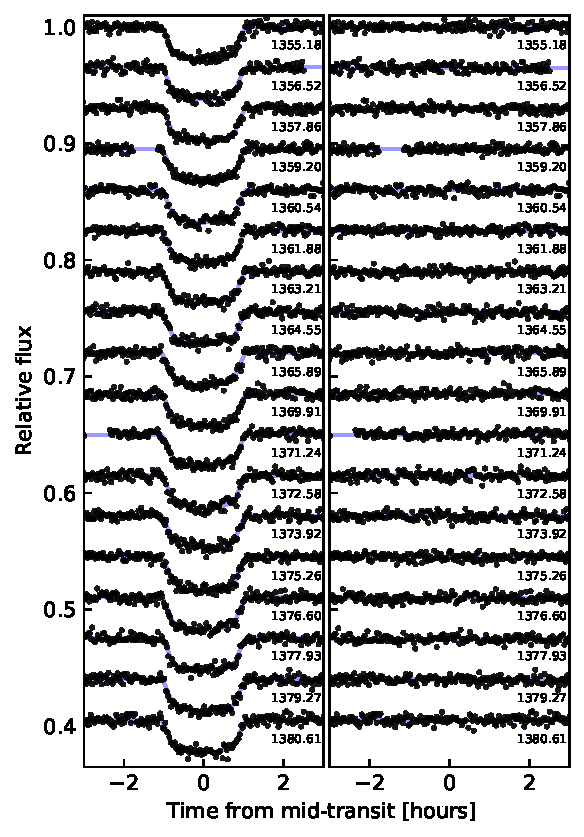
\includegraphics[width=0.5\textwidth]{f1.pdf}
	\end{center}
	\vspace{-0.7cm}
  \caption{ {\bf Timing residuals and best-fit models for WASP-4b.}
  The vertical axis shows the observed times minus the calculated
  times assuming a constant orbital period .  Darker points correspond
  to more precise data.  The quadratic ephemeris and its $1\sigma$
  uncertainties are shown in blue.  The binned TESS point (red square)
  is the weighted average of 18 TESS transits and is for display
  purposes only.  The models were fitted to all of the individual
  transit times.
  \label{fig:times}
	}
\end{figure}

We considered two possible models for the observed transit times.
The first model assumes a constant orbital period on a circular orbit:
\begin{align}
  t_{\rm tra}(E) &= t_0 + PE,\\
\end{align}
where $E$ is the epoch number and $t_0$ is a reference epoch.
The second model assumes the period changes at a steady rate:
\begin{align}
  t_{\rm tra}(E) &=
    t_0 + PE +
    \frac{1}{2} \frac{{\rm d}P}{{\rm d}E} E^2.
\end{align}
The free parameters are the reference epoch $t_0$, the period at
the reference epoch, and the period derivative, ${\rm d}P/{\rm d}t =
(1/P) {\rm d}P/{\rm d}E$.
We defined the epoch numbers such that $E=0$ is near the weighted
average of the observed times.  This helps to reduce the covariance
between $t_0$ and $P$.
A third possible model that we did not consider for reasons that will
become apparent is a precessing, eccentric orbit \citep[{\it
e.g.},][]{gimenez_revision_1995,patra_2017}.

We fitted each of the two models by assuming a Gaussian likelihood and
sampling over the posterior probability distributions.  We sampled the
posterior using the algorithm proposed by
\citet{goodman_ensemble_2010} and implemented by
\citet{foreman-mackey_emcee_2013} in \texttt{emcee}.  The prior for
the quadratic model allowed the period derivative to have any sign.

Figure~\ref{fig:times} shows the observed transit times, minus the
best-fit constant period model. 
The best-fitting constant-period model has $\chi^2 = XXX$ and YY
degrees of freedom.  The best-fitting
quadratic model has $\chi^2 = YYY$ and ZZ degrees of freedom. 
The difference in the BIC \citep{kass_bayes_1995} between the linear
and quadratic and models is $\Delta {\rm BIC} = ZZ.Z$, strongly
favoring the quadratic case.

The best-fit period derivative in the quadratic model is
\begin{equation}
\dot{P}
  = - (X.XX \pm 0.XX)\times 10^{-10}
  = - YY.Y \pm Z.Z~{\rm ms}\,{\rm yr}^{-1}.
  \label{eq:dP_dt_obs}
\end{equation}
This agrees with the value reported by \citet{southworth_transit_2019}
after their including an additional 22 archival transit measurements
($\dot{P} = - 9.2 \pm 1.1~{\rm ms}\,{\rm yr}^{-1}$).
It is smaller than the rate of period decrease found by
\citetalias{bouma_wasp4b_2019} ($- 12.6 \pm 1.2~{\rm ms}\,{\rm
yr}^{-1}$)., presumably because of missing coverage filled in by
\citeauthor{southworth_transit_2019}'s observations.
The other best-fit transit timing model parameters are reported in
{\bf Table~X}.



\subsection{Radial Velocities: WASP-4's acceleration towards the Earth}

%FIXME: is the purple here from my Pdot, or Southworth's?
%FIXME: perhaps include the WASP-4b phase-fold here too??
\begin{figure}[t]
	\begin{center}
		\leavevmode
		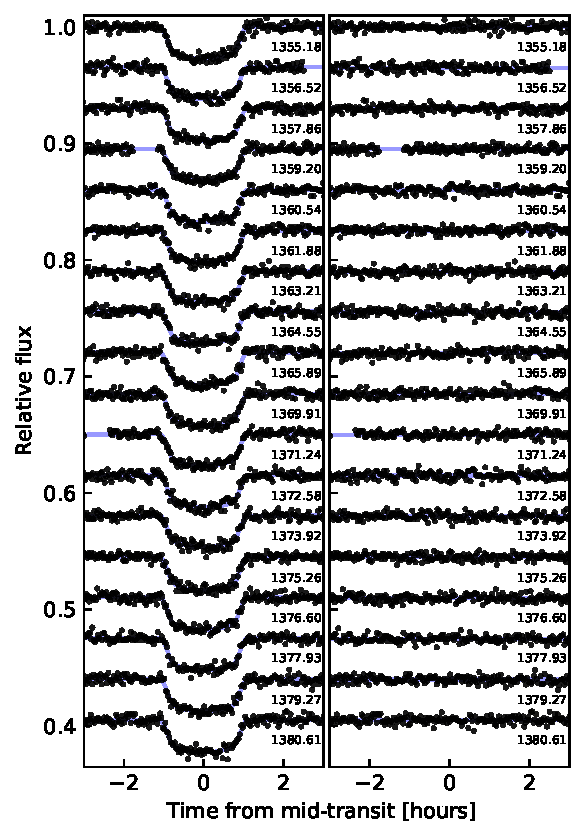
\includegraphics[width=0.5\textwidth]{f2.pdf}
	\end{center}
	\vspace{-0.7cm}
	\caption{
    {\bf Radial velocity observations of WASP-4.} The best-fit Keplerian orbit
    of WASP-4b has been subtracted.  The linear trend inferred from the
    RV data is shown with a black line, with $1\sigma$ errors in gray.
    The trend that would be needed to produce the period decrease seen
    in transits ($\dot{P}= - YY.Y \pm Z.Z~{\rm ms}\,{\rm yr}^{-1}$) is
    indicated with the purple dotted line.  The four new RV
    measurements presented in this work increased the significance of
    the slope from $\approx$2$\sigma$ to 15$\sigma$.
	\label{fig:rvs}
  \vspace{-0.3cm}
	}
\end{figure}

%FIXME: this entire paragraph copies Bouma+19 too heavily.
We began by fitting a single Keplerian orbit, plus instrument offsets,
jitters, and a long-term trend
\citep[][\texttt{radvel}]{fulton_radvel_2018}.  We set Gaussian priors
on the period and time of inferior conjunction using the values from
Table~4 of \citetalias{bouma_wasp4b_2019}, and fixed the eccentricity
to zero, per the results of \citet{beerer_secondary_2011},
\citet{knutson_friends_2014} and \citet{bonomo_gaps_2017}.  The free
parameters were the velocity semi-amplitude, the instrument
zero-points, the instrument jitters (an additive white noise term for
each instrument), linear ($\dot{v_{\rm r}}$), and optionally
second-order ($\ddot{v_{\rm r}}$) acceleration terms.

%FIXME: this is a janky approach if so??
We found that the best-fitting model with both linear and quadratic
radial velocity terms was marginally preferred (by $\Delta
\mathrm{BIC} = 5.8$) over the best-fitting model with only a linear
term.  Regardless, for consistency with \citet{knutson_friends_2014},
who fixed the quadratic component of the long-term trend to zero, in
Figure~\ref{fig:rvs} we show best-fitting models for the linear-trend
case.  

WASP-4 was found to be accelerating towards our line of sight at high
confidence,
\begin{equation}
  \dot{v}_{\rm r} =
     -0.0422^{+0.0028}_{-0.0027}
     \,{\rm m}\,{\rm s}^{-1}\,{\rm day}^{-1}.
\end{equation}
For comparison, before our recent observing run, 
$\dot{v}_{\rm r}$ was thought to be about five times smaller, and was
only marginally significant
\citep{knutson_friends_2014,bouma_wasp4b_2019}.

The system's acceleration towards our line of sight causes a decrease
in the apparent orbital period (the R{\o}mer delay).  The period
derivative expected from radial velocities is
\begin{align}
  \dot{P}_{\rm RV} &= \frac{\dot{v}_{\rm r} P}{c} \\
  \dot{P}_{\rm RV} &= -5.94 \pm 0.39~{\rm ms}\,{\rm yr}^{-1}.
\end{align}
In other words, the majority of the period decrease observed in
transits ($\dot{P} = - X.X \pm 1.1~{\rm ms}\,{\rm yr}^{-1}$) seems to
be explained by the acceleration of the host star.
% FIXME
All the
available TTV data show a period decrease of $\approx 8-12$
milliseconds per year~\citep{bouma_wasp-4b_2019,southworth_transit_2019,baluev_homogeneously_2019}.



An important consideration is whether the measured RV trend is at all
correlated with stellar activity.  We investigate this by analyzing
WASP-4's emission in the Ca II H \& K lines, as quantified with the
chromospheric $S$-index \citep{wright_chromospheric_2004}.  We only
examined the HIRES velocities for this step, since they are the main
source of signal for our analysis.  First, we subtracted the orbital
solution from the Keck-HIRES velocities.  Then, following
\citet{bryan_statistics_2016,bryan_excess_2019}, we calculated the
Spearman rank correlation coefficient between the $S$-index and the
orbit-subtracted velocities.  We found a correlation coefficient of
0.16. Though suggestive, it is not statistically significant (the
corresponding $p$-value is 0.65).  Furthermore, inspection of the
$S$-index timeseries showed no secular or sinusoidal trends, as would
be expected if we were observing a long-term magnetic activity cycle.
The $S$-index values are included in {\bf Table X}.  We conclude that
it would be highly unlikely for the linear trend to be caused by
stellar activity.


\subsection{Constraints on companion masses and semi-major axes}

%TODO: describe 3b better
%TODO: also, put 3b in as the bottom right inset to the contrast curve
\begin{figure}[!t]
	\gridline{
		\fig{f3a.png}{0.33\textwidth}{}
	}
	\vspace{-1cm}
	\gridline{
		\fig{f3b.pdf} {0.5\textwidth}{}
	}
	\vspace{-0.7cm}
    \caption{
      {\it Top:\,} 
      Speckle image reconstructed from 1000 40 millisecond frames in an 832 nm bandpass, and acquired on September 28, 2019.
      The image scale is $2.46''\times2.46''$.
      {\it Bottom:\,} 
      Contrast curve derived from point-source injection-recovery
      experiments.
    }
    \label{fig:zorro}
\end{figure}

\begin{figure}[t]
	\begin{center}
		\leavevmode
		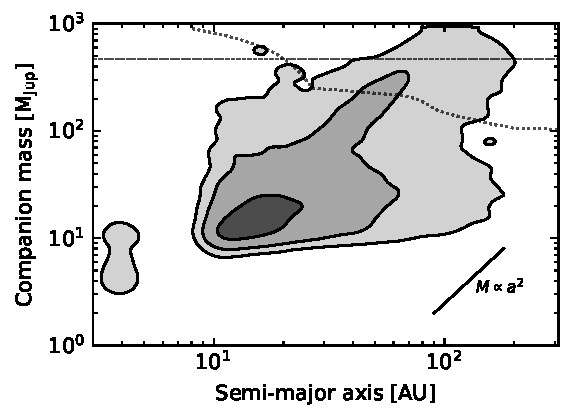
\includegraphics[width=0.48\textwidth]{f4.pdf}
	\end{center}
	\vspace{-0.7cm}
	\caption{
    {\bf Masses and semi-major axes of companions that meet
    requirements of both the radial velocity and the speckle imaging.}
    The likelihood inferred from radial velocities is shown in
    grayscale, and the region excluded from the imaging is shown with
    a cross-hatch pattern.
	\label{fig:mass_sma}
  \vspace{-0.3cm}
	}
\end{figure}


Given a linear radial velocity trend, we can place lower-limits on the
mass and semi-major axis of additional bodies in the system.  The
constraints on the two parameters are degenerate: $\dot{\gamma}
\propto M_{\rm p} a^{-2}$.  Nonetheless, the Zorro images and contrast
curves can limit the available parameter space by setting an upper
limit on the semimajor axis, and a maximum brightness (and thereby
mass) of any putative companions.

The general procedure we use to derive constraints on possible
companion masses and semi-major axes has been developed by
\citet{wright_linear_trends_2007}, \citet{crepp_trends_2012},
\citet{montet_trends_2014}, \citet{knutson_friends_2014},
\citet{bryan_statistics_2016,bryan_excess_2019}, and others.

\paragraph{Speckle imaging constraints}

First, we would like to convert the contrast ratios obtained through
the Zorro imaging (Figure~\ref{fig:zorro}) to limits on the masses of
putative companions and their separations from the host star.

To do this, we followed \citet{montet_trends_2014}, and opted to
employ the \citet{baraffe_evolutionary_2003} models for substellar
mass objects and the MIST isochrones for stellar mass objects
\citep{paxton_modules_2011,paxton_modules_2013,paxton_modules_2015,dotter_mesa_2016,choi_mesa_2016}.
We assumed that the system age was 5 Gyr, so that companions would
have fully contracted.

Due to the custom filters of the Zorro imager, and corresponding lack
of synthetic photometry, we further assumed that all sources had
blackbody spectra. While this is clearly false, we do not readily have
access to the planetary and stellar atmosphere models needed for the
consistent calculation with the \texttt{COND03} and \texttt{MESA}
models.  We therefore adopted the effective temperatures and
bolometric luminosities from the \citet{baraffe_evolutionary_2003} and
MIST isochrones.  Using these theoretical quantities and the empircal
Zorro bandpass functions, we calculated absolute magnitudes in the 562
and 832 nm Zorro bandpasses for stellar and planetary mass companions.
Applying the same calculation to WASP-4 itself using the effective
temperature and bolometric luminosity from
\citetalias{bouma_wasp4b_2019}, we derived the transformation from
contrast ratio to companion mass.
The resulting limits are shown as the cross-hatched region in
Figure~\ref{fig:mass_sma}.


\paragraph{Radial velocity constraints}

To derive constraints on possible companion masses and separations
from the radial velocities, we followed the procedure of
\citet{bryan_excess_2019}.  We began by defining a $50\times50$ grid
in true planetary mass and semimajor axis, evenly spaced from 1 to
300$\,$$M_{\rm Jup}$ and 3 to 500$\,$${\rm AU}$.  We then considered the
possibility that an additional companion in any particular cell could
explain the observed linear trend.  In each cell, we simulated 500
hypothetical companions.

We assigned each companion a mass and semimajor axis from log-uniform
distributions within the grid cell. We drew the inclination from a
uniform distribution in $\cos i$.  The eccentricity was drawn from
\citet{kipping_beta_2013}'s long-period exoplanet Beta distribution
($a=1.12$, $b=3.09$).  For each simulated companion, we then drew a
sample from the converged chains of our initial model of WASP-4b, plus
its linear trend. We subtracted the planet's orbital solution, leaving
the linear trend.  Given $(a_{\rm c}, M_{\rm c}, e_{\rm c}$ for each
simulated outer companion, and the fixed instrument offsets and
jitters from the MCMC chains, we then performed a maximum likelihood
fit for the time and argument of periastron of the outer simulated
companion.  We converted the resulting $50\times50\times500$ cube of
best-fit log-likelihood values to probabilities, and averaged over the
samples in each grid cell to derive a probability distribution in mass
and semi-major axis.

The result is shown as grayscale background in
Figure~\ref{fig:mass_sma}.



\section{Discussion}
\label{sec:discussion}

\subsection{Implications for WASP-4}
Previous possibilities suggested to explain the period decrease of
WASP-4b included tidal orbital decay, orbital precession, and
light-travel time effects \citep{bouma_wasp4b_2019}.  Our new radial
velocity measurements have now shown the least exotic
option---light-travel time effects---is also the most likely
explanation.  Transits show the obital period to decrease by $YY.Y \pm
Z.Z~{\rm ms}\,{\rm yr}^{-1}$; the line-of-sight acceleration observed
in radial velocities implies an expected period decrease of $YY.Y \pm
Z.Z~{\rm ms}\,{\rm yr}^{-1}$.  
Though the quantitative agreement is not perfect, Occam's razor would
suggest that the line of sight acceleration is probably a sufficient
explanation for the apparent decrease of WASP-4b's orbital period.
% While further radial velocity observations of the system should help
% in determining the mass and semi-major axis of the companion, it seems
% unlikely that additional transit observations will yield near-term
% constraints on orbital decay.

The corresponding requirements for the companion causing the
acceleration are that it is likely either a brown-dwarf or low mass
star, and that it is between $10$-$100\,{\rm AU}$ from the host star
(Figure~\ref{fig:mass_sma}).
Given such a mass, this companion could at one time have influenced
the orbital evolution of the inner giant.
Further radial velocity monitoring should eventually reveal the
orbital parameters and minimum mass of the companion.

\subsection{How many other hot Jupiters will show the R{\o}mer delay?}

We identified WASP-4b's decreasing orbital period as part of a search
for tidal orbital decay.  However, over half of hot Jupiters have
companions outside of $1\,{\rm AU}$ with super-Jovian masses
\citep{knutson_friends_2014}.  Line-of-sight accelerations are
therefore relatively common in hot Jupiter systems. 

To evaluate the importance of these effects in future transit timing
searches, we collected the linear trends reported by
\citet{knutson_friends_2014}, and computed the expected orbital period
derivatives $\dot{P}_{\rm RV} = \dot{v}_{\rm r} P/c$ for all the
systems.
The results are given in {\bf Table~X}, and visualized for hot
Jupiters with significant linear trends in Figure~\ref{fig:pdot_pop}.

\begin{figure}[t]
	\begin{center}
		\leavevmode
		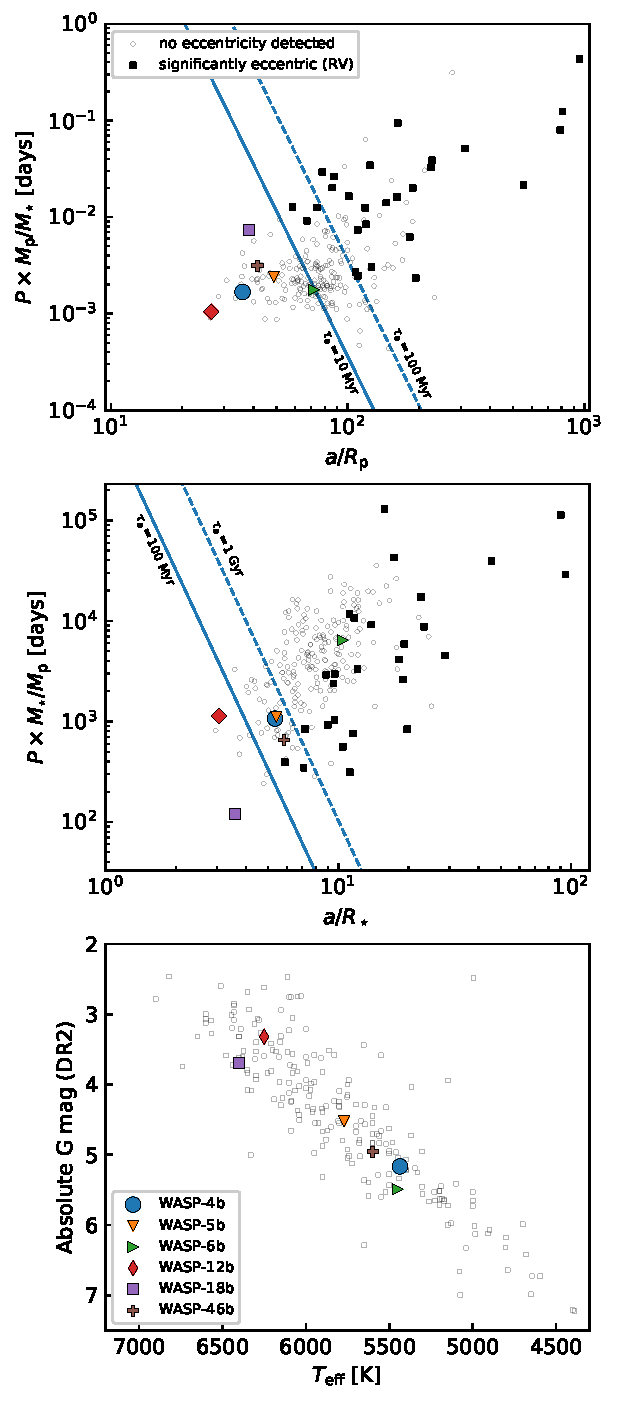
\includegraphics[width=0.48\textwidth]{f5.pdf}
	\end{center}
	\vspace{-0.7cm}
	\caption{
  {\bf Predicted hot Jupiter period changes from linear radial
  velocity trends.} Including WASP-4b, 16 of 51 hot Jupiters from
  \citet{knutson_friends_2014} have shown long-term radial velocity
  trends.  The HAT-P-11 signal is plotted, though its radial velocity
  signal may be caused by stellar activity.  Three hot Jupiters are
  not plotted because their radial velocity curves better described as
  quadratic trends in time: HAT-P-17, WASP-8, and WASP-34.  Objects
  are ordered in the $y$ dimension by the absolute value of d$P$/d$t$.
	\label{fig:pdot_pop}
  \vspace{-0.3cm}
	}
\end{figure}


\section{Conclusions}
\label{sec:conclusions}

We found that WASP-4 is accelerating towards the Earth, at
X.XX m/s/yr.
This seems like the most plausible explanation for the orbital 
period decrease observed in transits~---~not tidal
orbital decay, or apsidal precession.
The most likely parameters for the companion are XXX.
Over half of hot Jupiters have super-Jovian outer companions,
so the R{\o}mer delay will become an increasingly large nuisance in
the hunt for orbital decay as
the observing baselines for hot Jupiters increase.
The requirement to avoid missing out is to have long-term
radial velocity monitoring with the same spectrograph (or else to
calibrate instrumental offsets by observing the same stars simultaneously).

%TODO: what's the scaling? sigma_P ~ 1/baseline? baseline^2?


%%%%%%%%%%%%%%%%%%%%%%%%%%%%%%%%%%%%%%%%%%%%%%%%%%%%%%%%%%%%%%%%%%%%%%%%%%%%%%%

% \acknowledgements
% %
% This paper includes data collected by the TESS mission, which are
% publicly available from the Mikulski Archive for Space Telescopes
% (MAST).
% %
% Funding for the TESS mission is provided by NASA's Science Mission
% directorate.
% %
% This work made use of NASA's Astrophysics Data System Bibliographic
% Services.
% %
% Based on observations obtained at the Gemini Observatory, which is
% operated by the Association of Universities for Research in Astronomy,
% Inc., under a cooperative agreement with the NSF on behalf of the
% Gemini partnership: the National Science Foundation (United States),
% National Research Council (Canada), CONICYT (Chile), Ministerio de
% Ciencia, Tecnolog\'{i}a e Innovaci\'{o}n Productiva (Argentina),
% Minist\'{e}rio da Ci\^{e}ncia, Tecnologia e Inova\c{c}\~{a}o (Brazil),
% and Korea Astronomy and Space Science Institute (Republic of Korea).
% %
% Observations in the paper made use of the High-Resolution Imaging
% instrument Zorro at Gemini-South. Zorro was funded by the NASA
% Exoplanet Exploration Program and built at the NASA Ames Research
% Center by Steve B. Howell, Nic Scott, Elliott P. Horch, and Emmett
% Quigley.
% %
% This research has made use of the VizieR catalogue access tool, CDS,
% Strasbourg, France. The original description of the VizieR service was
% published in A\&AS 143, 23.
% %
% This work has made use of data from the European Space Agency (ESA)
% mission {\it Gaia} (\url{https://www.cosmos.esa.int/gaia}), processed
% by the {\it Gaia} Data Processing and Analysis Consortium (DPAC,
% \url{https://www.cosmos.esa.int/web/gaia/dpac/consortium}). Funding
% for the DPAC has been provided by national institutions, in particular
% the institutions participating in the {\it Gaia} Multilateral
% Agreement.
%
% \newline
%

\software{
  \texttt{astrobase} \citep{bhatti_astrobase_2018},
	\texttt{astroplan} \citep{astroplan2018},
  \texttt{astropy} \citep{the_astropy_collaboration_astropy_2018},
  \texttt{astroquery} \citep{astroquery_2018},
  % \texttt{BATMAN} \citep{kreidberg_batman_2015},
  \texttt{corner} \citep{corner_2016},
  \texttt{emcee} \citep{foreman-mackey_emcee_2013},
  \texttt{IPython} \citep{perez_2007},
  \texttt{matplotlib} \citep{hunter_matplotlib_2007}, 
	\texttt{MESA} \citep{paxton_modules_2011,paxton_modules_2013,paxton_modules_2015}
  \texttt{numpy} \citep{walt_numpy_2011}, 
  \texttt{pandas} \citep{mckinney-proc-scipy-2010},
  \texttt{radvel} \citep{fulton_radvel_2018},
  % \texttt{scikit-learn} \citep{scikit-learn},
  \texttt{scipy} \citep{jones_scipy_2001}.
}

%\clearpage
%\newpage
%\renewcommand{\arraystretch}{1.0}

\startlongtable
\begin{deluxetable}{lc}

\tabletypesize{\footnotesize}

\tablenum{4}

%\tablewidth{0pt}

\tablecaption{Best-fit model parameters.}
\label{tab:bestfit}

\tablehead{
  \colhead{Parameter} &
  \colhead{Median Value~(Unc.)\tablenotemark{a}}
}

\startdata
~~~~~~{\it Constant period} &  \\
$t_0$\,[${\rm BJD}_{\rm TBD}$]    & 2455804.515752(+19)(-19)              \\
$P$\,[days]                       & 1.338231466(+23)(-22)                 \\
~~~~~~{\it Constant period derivative} &  \\
$t_0$~[${\rm BJD}_{\rm TBD}$]     & 2455804.515918(+24)(-24)              \\
$P$\,[days]                       & 1.338231679(+31)(-31)                 \\
$dP/dt$                           & $-4.00(+37)(-38) \times 10^{-10}$     \\
~~~~~~{\it Apsidal precession} &  \\
$t_0$~[${\rm BJD}_{\rm TBD}$]     & 2455804.51530(+25)(-31)               \\
$P_{\rm s}$\,[days]               & 1.33823127(+20)(-48)                  \\
$e$                               & $1.92^{+1.93}_{-0.76} \times 10^{-3}$ \\
$\omega_0$\,[rad]                 & 2.40(+38)(-34)                        \\
$d\omega/dE$~[rad\,epoch$^{-1}$]  & $8.70^{+3.01}_{-2.30} \times 10^{-4}$ \\
\enddata
\tablenotetext{a}{
The numbers in parenthesis give the $68\%$ confidence interval for the final
two digits, where appropriate.
}
\end{deluxetable}




\bibliographystyle{yahapj}                            
\bibliography{bibliography} 

\end{document}
